% +------------------------------------------------------------------------+
% | Reference manual page: Triangulation_3.tex
% +------------------------------------------------------------------------+
% | 27.3.2000   Monique Teillaud
% | Package: Triangulation3
% | 
\RCSdef{\RCSTriangulationRev}{$Revision$}
\RCSdefDate{\RCSTriangulationDate}{$Date$}
% |
%%RefPage: end of header, begin of main body
% +------------------------------------------------------------------------+


\begin{ccRefClass}{Triangulation_3<TriangulationTraits_3,TriangulationDataStructure_3>}  %% add template arg's if necessary

%% \ccHtmlCrossLink{}     %% add further rules for cross referencing links
%% \ccHtmlIndexC[class]{} %% add further index entries

\ccDefinition
  
The class \ccRefName\ expects a model of a \ccc{geometric traits
class} as its first template argument and a model of a \ccc{triangulation data
structure} as its second argument. 

The second argument is optional,
since a default parameter is proposed by \cgal. This default parameter
is
\ccc{Triangulation_data_structure_3< Triangulation_vertex_base_3<TriangulationTraits_3>,Triangulation_cell_base_3<TriangulationTraits_3> 
>}. 


\ccInclude{CGAL/Triangulation_3.h}

\ccInheritsFrom{\ccc{Triangulation_utils_3}}

\ccTypes
The class \ccClassTemplateName\ defines the following types:
\ccThree{typedef TriangulationTraits_3::Tetrahedron Tetrahedron;}
{Tetrahedron}{}
\ccThreeToTwo

\ccTypedef{typedef TriangulationDataStructure_3 Triangulation_data_structure;}{}
\ccGlue
\ccTypedef{typedef TriangulationTraits_3 Geom_traits;}{}

\ccTypedef{typedef TriangulationTraits_3::Point_3 Point;}{}
\ccGlue
\ccTypedef{typedef TriangulationTraits_3::Segment_3 Segment;}{}
\ccGlue
\ccTypedef{typedef TriangulationTraits_3::Triangle_3 Triangle;}{}
\ccGlue
\ccTypedef{typedef TriangulationTraits_3::Tetrahedron_3 Tetrahedron;}{}

Only vertices ($0$-faces) and cells ($3$-faces) are stored. Edges
($1$-faces) and facets ($2$-faces) are not explicitly represented and
thus there are no corresponding classes (see
Section~\ref{Triangulation3-sec-intro}).

\ccNestedType{Vertex}{Vertex type}
\ccGlue
\ccNestedType{Cell}{Cell type}

\ccTypedef{typedef pair<Cell_handle, int> Facet;}{Facet type.
The pair \ccc{(c,i)} denotes facet on index \ccc{i} in cell \ccc{c}.}
\ccGlue
\ccTypedef{typedef triple<Cell_handle, int, int> Edge;}{Edge type.
The triple \ccc{Edge(c,i,j)} denotes the edge with vertices of index
\ccc{i} and \ccc{j} in cell \ccc{c}.}

The vertices and faces of the triangulations are accessed through
\ccc{handles}, \ccc{iterators} and \ccc{circulators}. 
A handle is a type which supports the two dereference operators
\ccc{operator*} and \ccc{operator->}. Iterator and circulators are
bidirectional and non-mutable.  Circulators and iterators are
assignable to the corresponding handle types. Whenever a handle appears 
in the parameter list of a function, an appropriate iterator or
circulator can be used as well \textit{(not yet implemented)}.  The
edges and facets of the 
triangulation can also be visited through iterators and circulators
which are bidirectional and non-mutable.

\ccNestedType{Vertex_handle}{handle to a vertex}
\ccGlue
\ccNestedType{Cell_handle}{handle to a cell}

\ccNestedType{Cell_iterator}{iterator over cells}
\ccGlue
\ccNestedType{Facet_iterator}{iterator over facets}
\ccGlue
\ccNestedType{Edge_iterator}{iterator over edges}
\ccGlue
\ccNestedType{Vertex_iterator}{iterator over vertices}

\ccNestedType{Finite_cells_iterator}{iterator over finite cells}
\ccGlue
\ccNestedType{Finite_facets_iterator}{iterator over finite facets}
\ccGlue
\ccNestedType{Finite_edges_iterator}{iterator over finite edges}
\ccGlue
\ccNestedType{Finite_vertices_iterator}{iterator over finite vertices}

\ccNestedType{Cell_circulator}{circulator over all cells incident to a
given edge} 
\ccGlue
\ccNestedType{Facet_circulator}{circulator over all facets incident to a
given edge}

The triangulation class also defines the following enum type to specify
which case occurs when locating a point in the triangulation. 

\ccEnum{enum Locate_type {VERTEX=0, EDGE, FACET, CELL, OUTSIDE_CONVEX_HULL, 
OUTSIDE_AFFINE_HULL};}
{}


\ccCreation
\ccCreationVariable{t}  %% choose variable name

\ccThree{Triangulation_3<>}{Facet }{}

\ccConstructor{Triangulation_3<TriangulationTraits_3,TriangulationDataStructure_3>
(const TriangulationTraits_3 & traits );}
{Introduces a triangulation \ccVar\ having only one vertex which is the
infinite vertex.} 

\ccConstructor{Triangulation_3<TriangulationTraits_3,TriangulationDataStructure_3>(const
Triangulation_3<TriangulationTraits_3,TriangulationDataStructure_3> & tr);} 
{Copy constructor. All vertices and faces are duplicated.}

\ccFunction{void ~t();}
{Destructor. All vertices (including the infinite vertex) and cells are
deleted.}

\ccOperations

\ccHeading{Assignment}

\ccMethod{Triangulation_3<TriangulationTraits_3,TriangulationDataStructure_3>
	operator=(const Triangulation_3<TriangulationTraits_3,TriangulationDataStructure_3> & tr);}
{The triangulation \ccc{tr} is duplicated, and modifying one copy after the 
duplication does not modify the other copy.}

\ccMethod{void copy_triangulation
		(const Triangulation_3<TriangulationTraits_3,TriangulationDataStructure_3> & tr);}
{The triangulation is duplicated.}

The previous two methods are equivalent.

\ccMethod{void swap(Triangulation_3<TriangulationTraits_3,TriangulationDataStructure_3> & tr);}
{The triangulations \ccc{tr} and \ccVar\ are swapped.
\ccVar.\ccc{swap(tr)} should be preferred to \ccVar\ = \ccc{tr} or to
\ccc{t(tr)} if \ccc{tr} is deleted after that. Indeed, there is no
copy of cells and vertices, thus this method runs in constant time.}

\ccAccessFunctions
\ccThree{Vertex_handle}{t.number_of_finite_edges()toto}{}

\ccMethod{const TriangulationTraits_3 & geom_traits() const;}
{Returns a const reference to the geometric traits object.}
\ccGlue
\ccMethod{const TriangulationDataStructure_3 & tds() const;}
{Returns a const reference to the triangulation data structure.}

\ccMethod{int dimension() const;}
{Returns the dimension of the affine hull.}
\ccGlue
\ccMethod{int number_of_vertices() const;}
{Returns the number of finite vertices.}

\ccMethod{Vertex_handle infinite_vertex();}
{Returns the infinite vertex.}
\ccGlue
\ccMethod{Cell_handle infinite_cell() const;}
{Returns a cell incident to the infinite vertex.}

\ccHeading{Non-constant-time access functions}

As previously said, the triangulation is a collection of cells that
are either infinite or represent a finite tetrahedra, where an
infinite cell is a 
cell incident to the infinite vertex. Similarly we call
an edge (resp. facet) \ccc{infinite} if it is incident to the infinite vertex.

\ccMethod{int number_of_cells() const;}
{The number of cells. Returns 0 if \ccVar.\ccc{dimension()}$<3$.}
\ccGlue
\ccMethod{int number_of_facets() const;}
{The number of facets. Returns 0 if \ccVar.\ccc{dimension()}$<2$.}
\ccGlue
\ccMethod{int number_of_edges() const;}
{The number of edges. Returns 0 if \ccVar.\ccc{dimension()}$<1$.}

\ccMethod{int number_of_finite_cells() const;}
{The number of finite cells. Returns 0 if \ccVar.\ccc{dimension()}$<3$.}
\ccGlue
\ccMethod{int number_of_finite_facets() const;}
{The number of finite facets. Returns 0 if \ccVar.\ccc{dimension()}$<2$.}
\ccGlue
\ccMethod{int number_of_finite_edges() const;}
{The number of finite edges. Returns 0 if \ccVar.\ccc{dimension()}$<1$.}

\begin{ccAdvanced}
\ccHeading{Setting}
\ccMethod{void set_number_of_vertices(int n);}
{Sets the number of vertices to \ccc{n}.}
\end{ccAdvanced}

\ccHeading{Geometric access functions}
\ccThree{Tetrahedron}{t.tetrahedron()}{}

\ccMethod{Tetrahedron tetrahedron(const Cell_handle c) const;}
{Returns the tetrahedron formed by the four vertices of \ccc{c}.
\ccPrecond{\ccVar.\ccc{dimension()} $=3$ and the cell is finite.}}
\ccGlue
\ccMethod{Triangle triangle(const Facet & f) const;}
{Returns the triangle formed by the three vertices of \ccc{f}. 
\ccPrecond{\ccVar.\ccc{dimension()} $\geq 2$ and the facet is finite.}}
\ccGlue
\ccMethod{Triangle triangle(const Cell_handle c, int i) const;}
{Same as the previous method for facet \ccc{(c,i)}.
\ccPrecond{As above and $i \in \{0,1,2,3\}$ in dimension~3, $i = 3$ in
dimension~2.}}
\ccGlue
\ccMethod{Segment segment(const Edge & e) const;}
{Returns the line segment formed by the vertices of \ccc{e}.
\ccPrecond{\ccVar.\ccc{dimension()} $\geq 1$ and \ccc{e} is finite.}}
\ccGlue
\ccMethod{Segment segment(const Cell_handle c, int i, int j) const;}
{Same as the previous method for edge \ccc{(c,i,j)}.
\ccPrecond{As above and $i\neq j$. Moreover $i,j \in \{0,1,2,3\}$ in
dimension~3, $i,j \in \{0,1,2\}$ in dimension~2, $i,j \in \{0,1\}$ in 
dimension~1.}}

 \textit{not yet implemented : geometric access functions with iterators or
circulators as arguments.}

\ccHeading{Tests for Finite and Infinite Vertices and Faces}

\ccMethod{bool is_infinite(const Vertex_handle v) const;}
{\ccc{true}, iff vertex \ccc{v} is the infinite vertex.}
\ccGlue
\ccMethod{bool is_infinite(const Cell_handle c) const;}
{\ccc{true}, iff \ccc{c} is incident to the infinite vertex.
\ccPrecond{\ccVar.\ccc{dimension()} $=3$.}}
\ccGlue
\ccMethod{bool is_infinite(const Cell_handle c, int i) const;}
{\ccc{true}, iff the facet \ccc{i} of cell \ccc{c} is incident to the
infinite vertex.
\ccPrecond{\ccVar.\ccc{dimension()} $\geq 2$ and $i\in\{0,1,2,3\}$ in
dimension~3, $i=3$ in dimension~2.}} 
\ccGlue
\ccMethod{bool is_infinite(const Facet & f) const;}
{\ccc{true} iff facet \ccc{f} is incident to the infinite vertex.
\ccPrecond{\ccVar.\ccc{dimension()} $\geq 2$.}}
\ccGlue
\ccMethod{bool is_infinite(const Cell_handle c, int i, int j) const;}
{\ccc{true}, iff the edge \ccc{(i,j)} of cell \ccc{c} is incident to
the infinite vertex.
\ccPrecond{\ccVar.\ccc{dimension()} $\geq 1$ and $i\neq j$. Moreover
$i,j \in \{0,1,2,3\}$ in dimension~3, $i,j \in \{0,1,2\}$ in dimension
2, $i,j \in \{0,1\}$ in  dimension~1.}} 
\ccGlue
\ccMethod{bool is_infinite(const Edge & e) const;}
{\ccc{true} iff edge \ccc{e} is incident to the infinite vertex.
\ccPrecond{\ccVar.\ccc{dimension()} $\geq 1$.}}

\ccHeading{Queries}

\ccMethod{bool is_vertex(const Point & p, Vertex_handle & v) const;}
{Tests whether \ccc{p} is a vertex of \ccVar\ by locating \ccc{p} in
the triangulation. If \ccc{p} is found, the associated vertex \ccc{v}
is given.}
\ccGlue
\ccMethod{bool is_vertex(Vertex_handle v) const;}
{Tests whether \ccc{v} is a vertex of \ccVar.}

\ccMethod{bool is_edge(Vertex_handle u, Vertex_handle v, 
			Cell_handle & c, int & i, int & j) const;}
{Tests whether \ccc{(u,v)} is an edge of \ccVar. If the edge is found,
it gives a cell \ccc{c} having this edge and the indices \ccc{i}
and \ccc{j} of the vertices \ccc{u} and \ccc{v} in \ccc{c}, in this order.  
\ccPrecond{\ccc{u} and \ccc{v} are vertices of \ccVar.}}

\ccMethod{bool is_facet(Vertex_handle u, Vertex_handle v, Vertex_handle w, 
			Cell_handle & c, int & i, int & j, int & k) const;}
{Tests whether \ccc{(u,v,w)} is a facet of \ccVar. If the facet is found,
it computes a cell \ccc{c} having this facet and the indices \ccc{i},
\ccc{j} and \ccc{k} of the vertices \ccc{u}, \ccc{v} and \ccc{w} in \ccc{c}, 
in this order.  
\ccPrecond{\ccc{u}, \ccc{v} and \ccc{w} are vertices of \ccVar.}}

\ccMethod{bool is_cell(Cell_handle c) const;}
{Tests whether \ccc{c} is a cell of \ccVar.}
\ccGlue
\ccMethod{bool is_cell(Vertex_handle u, Vertex_handle v, 
			Vertex_handle w, Vertex_handle x,
			Cell_handle & c, 
			int & i, int & j, int & k, int & l) const;}
{Tests whether \ccc{(u,v,w,x)} is a cell of \ccVar. 
If the cell \ccc{c} is found, the method
computes the indices \ccc{i}, \ccc{j}, \ccc{k} and \ccc{l} of the
vertices \ccc{u}, \ccc{v}, \ccc{w} and \ccc{x} in \ccc{c}, in this
order. 
\ccPrecond{\ccc{u}, \ccc{v}, \ccc{w} and \ccc{x} are vertices of \ccVar.}}
\ccGlue
\ccMethod{bool is_cell(Vertex_handle u, Vertex_handle v, 
			Vertex_handle w, Vertex_handle x,
			Cell_handle & c) const;}
{Tests whether \ccc{(u,v,w,x)} is a cell of \ccVar\ and computes 
this cell \ccc{c}.
\ccPrecond{\ccc{u}, \ccc{v}, \ccc{w} and \ccc{x} are vertices of \ccVar.}}

There is a method \ccc{has_vertex} in the cell class. The analogous
methods for facets are defined here.

\ccMethod{bool has_vertex(const Facet & f, Vertex_handle v, int & j) const;}
{If \ccc{v} is a vertex of \ccc{f}, then \ccc{j} is the index of
\ccc{v} in the cell \ccc{f.first}, and the method returns \ccc{true}.
\ccPrecond{\ccVar.dimension()==3}}
\ccGlue
\ccMethod{bool has_vertex(Cell_handle c, int i, 
	Vertex_handle v, int & j) const;}
{Same for facet \ccc{(c,i)}. Computes the index \ccc{j} of \ccc{v} in
\ccc{c}.}
\ccGlue
\ccMethod{bool has_vertex(const Facet & f, Vertex_handle v) const;}
{}
\ccGlue
\ccMethod{bool has_vertex(Cell_handle c, int i, Vertex_handle v) const;}
{Same as the first two methods, but these two methods do not return the
index of the vertex.}

The following three methods test whether two facets have the same
vertices.

\ccMethod{bool are_equal(Cell_handle c, int i, Cell_handle n, int j) const;}
{}
\ccGlue
\ccMethod{bool are_equal(const Facet & f, const Facet & g) const;}
{}
\ccGlue
\ccMethod{bool are_equal(const Facet & f, Cell_handle n, int j) const;}
{For these three methods: \ccPrecond{\ccVar.dimension()==3}.}


\ccHeading{Point location}
\ccThree{Vertex_handle}{t.locate()toto}{}

The class \ccClassTemplateName\  provides two functions to locate
a given point with respect to a triangulation. It provides
also functions to test if a given point is inside a finite face
or not.

\ccMethod{Cell_handle
          locate(const Point & query, Cell_handle start = NULL) const;}
{
%\ccPrecond{\ccVar.\ccc{dimension()} $= 3$ (otherwise there is no
%cell yet).}\\
If the point \ccc{query} lies inside the convex hull of the points, the cell 
that contains the query in its interior is returned. If \ccc{query} lies on a
facet, an edge or on a vertex, one of the cells having \ccc{query} on
its boundary is returned.\\ 
If the point \ccc{query} lies outside the convex hull of the points,
an infinite cell with vertices $\{ p, q, r, \infty\}$ is returned such that
the tetrahedron $( p, q, r, query )$ is positively oriented
(the rest of the triangulation lies on the other side of facet 
$( p, q, r )$). \\
Note that locate works even in degenerate dimensions: in dimension 2
(resp. 1, 0) the \ccc{Cell_handle} returned is the one that represents
the facet (resp. edge, vertex) containing the query point. \\
The optional argument \ccc{start} is used as a starting place for the search.
}

\ccMethod{Cell_handle
          locate(const Point & query, Locate_type & lt,
                 int & li, int & lj, Cell_handle start = NULL ) const;}
{If \ccc{query} lies inside the affine hull of the points, the $k$-face
(finite or infinite) that contains \ccc{query} in its interior is
returned, by means of the cell returned together with \ccc{lt}, which
is set to the locate type of the query (\ccc{VERTEX, EDGE, FACET,
CELL}, or \ccc{OUTSIDE_CONVEX_HULL} if the cell is infinite and \ccc{query}
lies strictly in it) and two indices \ccc{li} and \ccc{lj} that
specify the $k$-face of the cell containing \ccc{query}.\\ 
If the $k$-face is a cell, \ccc{li} and \ccc{lj} have no
meaning; if it is a facet (resp. vertex), \ccc{li} gives the index of
the facet (resp. vertex) and \ccc{lj} has no meaning; if it is and
edge, \ccc{li} and \ccc{lj} give the indices of its vertices.\\ 
%If the point \ccc{query} lies outside the convex hull of the points, but 
%in their affine hull, then \ccc{lt} is set to \ccc{OUTSIDE_CONVEX_HULL}, 
%and a $k$-face separating the triangulation from \ccc{query} is
%specified by the cell containing \ccc{query}, which is returned, and
%indices as previously.\\
If the point \ccc{query} lies outside the affine hull of the points,
which can happen in case of degenerate dimensions, \ccc{lt} is set to
\ccc{OUTSIDE_AFFINE_HULL}, and the cell returned has no meaning.
As a particular case, if there is no finite vertex yet in the
triangulation, \ccc{lt} is set to \ccc{OUTSIDE_AFFINE_HULL} and
\ccc{locate} returns \ccc{NULL}. \\
The optional argument \ccc{start} is used as a starting place for the search.
}

\ccMethod{Bounded_side
          side_of_cell(const Point & p,
			Cell_handle c,
                        Locate_type & lt, int & li, int & lj) const;}
{Returns a value indicating on which side of the oriented boundary
of \ccc{c} the point \ccc{p} lies. More precisely, it returns:\\
- \ccc{ON_BOUNDED_SIDE} if \ccc{p} is inside the cell. For an infinite
cell this means that \ccc{p} lies strictly in the half space limited by
its finite facet and not containing any other point of the triangulation. \\
- \ccc{ON_BOUNDARY} if p on the boundary of the cell. For an infinite
cell this means that \ccc{p} lies on the \textit{finite} facet. Then
\ccc{lt} together with \ccc{li} and \ccc{lj} give the precise location
on the boundary. (See the descriptions of the \ccc{locate} methods.)\\ 
- \ccc{ON_UNBOUNDED_SIDE} if \ccc{p} lies outside the cell. For an
infinite cell this means that \ccc{p} does not satisfy either of the
two previous conditions.  
\ccPrecond{\ccVar.\ccc{dimension()} $=3$}}

\ccMethod{Bounded_side
          side_of_facet(const Point & p,
			const Facet & f,
			Locate_type & lt, int & li, int & lj) const;}
{Returns a value indicating on which side of the oriented boundary
of \ccc{f} the point \ccc{p} lies:\\
- \ccc{ON_BOUNDED_SIDE} if \ccc{p} is inside the facet. For an
infinite facet this means that \ccc{p} lies strictly in the half plane
limited by its finite edge and not containing any other point of the
triangulation . \\
- \ccc{ON_BOUNDARY} if \ccc{p} is on the boundary of the facet.
For an infinite facet this means that \ccc{p} lies on the finite
edge. \ccc{lt}, \ccc{li} and \ccc{lj} give the precise location of
\ccc{p} on the boundary of the facet. \ccc{li} and \ccc{lj} refer to
indices in the degenerate cell \ccc{c} representing \ccc{f}.\\
- \ccc{ON_UNBOUNDED_SIDE} if \ccc{p} lies outside the facet. For
an infinite facet this means that \ccc{p} does not satisfy either of
the two previous conditions. \\
\ccPrecond{\ccVar.\ccc{dimension()} $=2$ and \ccc{p} lies in the
plane containing the triangulation. \ccc{f.second} $=3$ (in dimension~2 
there is only one facet per cell).}}
\ccGlue
\ccMethod{Bounded_side
          side_of_facet(const Point & p,
			Cell_handle c, 
                        Locate_type & lt, int & li, int & lj) const;}
{Same as the previous method for the facet \ccc{(c,3)}.}

\ccMethod{Bounded_side
          side_of_edge(const Point & p, 
			const Edge & e,
                        Locate_type & lt, int & li) const;}
{Returns a value indicating on which side of the oriented boundary
of \ccc{e} the point \ccc{p} lies:\\
- \ccc{ON_BOUNDED_SIDE} if \ccc{p} is inside the edge. For an
infinite edge this means that \ccc{p} lies in the half line defined by
the vertex and not containing any other point of the triangulation.\\ 
- \ccc{ON_BOUNDARY} if \ccc{p} equals one of the vertices,
\ccc{li} give the index of the vertex in the cell storing \ccc{e}\\
- \ccc{ON_UNBOUNDED_SIDE} if \ccc{p} lies outside the edge. For
an infinite edge this means that \ccc{p} lies on the other half line,
which contains the other points of the triangulation.
\ccPrecond{\ccVar.\ccc{dimension()} $=1$ and \ccc{p} is collinear
with the points of the triangulation. \ccc{e.second} $=0$ and
\ccc{e.third} $=1$ (in dimension~1 there is only one edge per cell).}}
\ccGlue
\ccMethod{Bounded_side
          side_of_edge(const Point & p,
			Cell_handle c, 
                        Locate_type & lt, int & li) const;}
{Same as the previous method for edge $(c,0,1)$.}

\ccHeading{Flips}

Two kinds of flips exist for a three-dimensional triangulation. They
are reciprocal. To be flipped, an edge must be incident to three
tetrahedra. During the flip, these three tetrahedra disappear and two
tetrahedra appear. Figure~\ref{Triangulation3-fig-flips}(left) shows the
edge that is flipped as bold dashed, and one of its three incident
facets is shaded. On the right, the facet shared by the two new
tetrahedra is dashed. 

Flips are possible only under the following conditions:\\
- the edge or facet to be flipped is not on the boundary of the convex
hull of the triangulation 
- the points that will be vertices of the tetrahedra to be created are 
in convex position.

\begin{figure}
\begin{ccTexOnly}
\begin{center} 

\includegraphics{flips.eps}
\end{center}
\end{ccTexOnly}
\caption{Flips.
\label{Triangulation3-fig-flips}}
\begin{ccHtmlOnly}
<CENTER>
<img border=0 src="./flips.gif" align=center
alt="Flips">
</CENTER>
\end{ccHtmlOnly}
\end{figure} 

The following methods guarantee the validity of the resulting 3D
triangulation.

\textit{Flips for a 2d triangulation are not implemented yet}

\ccMethod{bool flip(Edge e);}
\ccGlue
\ccMethod{bool flip(Cell_handle c, int i, int j);}
{Before flipping, these methods check that edge \ccc{e=(c,i,j)} is
flippable (which is quite expensive). They return \ccc{false} or
\ccc{true} according to this test.}

\ccMethod{void flip_flippable(Edge e);}
\ccGlue
\ccMethod{void flip_flippable(Cell_handle c, int i, int j);}
{Should be preferred to the previous methods when the edge is
known to be flippable.
\ccPrecond{The edge is flippable.}}

\ccMethod{bool flip(Facet f);}
\ccGlue
\ccMethod{bool flip(Cell_handle c, int i);}
{Before flipping, these methods check that facet \ccc{f=(c,i)} is
flippable (which is quite expensive). They return \ccc{false} or
\ccc{true} according to this test.} 

\ccMethod{void flip_flippable(Facet f);}
\ccGlue
\ccMethod{void flip_flippable(Cell_handle c, int i);}
{Should be preferred to the previous methods when the facet is
known to be flippable.
\ccPrecond{The facet is flippable.}}

\ccHeading{Insertions}

The following operations are guaranteed to lead to a valid triangulation 
when they are applied on a valid triangulation.

\ccMethod{Vertex_handle insert(const Point & p, Cell_handle start = NULL );}
{Inserts point \ccc{p} in the triangulation and returns the corresponding
 vertex.\\
If point \ccc{p} coincides with an already existing vertex, this 
vertex is returned and the triangulation remains unchanged.\\
If point \ccc{p} lies in the convex hull of the points, it is added
naturally: if it lies inside a cell, the cell is split into four
cells, if it lies on a facet, the two incident cells are split into
three cells, if it lies on an edge, all the cells incident to this
edge are split into two cells.\\
If point \ccc{p} is strictly outside the convex hull but in the affine
hull, \ccc{p} is linked to all visible points on the convex hull to
form the new triangulation. See
Figure~\ref{Triangulation3-fig-insert_outside_convex_hull}.\\  
If point \ccc{p} is outside the affine hull of the points, \ccc{p} is
linked to all the points, and the dimension of the triangulation is
incremented. All the points now belong to the boundary of the convex
hull, so, the infinite vertex is linked to all the points to
triangulate the new infinite face. See 
Figure~\ref{Triangulation3-fig-insert_outside_affine_hull}.
The optional argument \ccc{start} is used as a starting place for the search.}

\ccMethod{template < class InputIterator >
          int
          insert(InputIterator first, InputIterator last);}
{Inserts the points in the range $\left[\right.$\ccc{first},
\ccc{last}$\left.\right)$.  Returns the number of inserted points.
\ccPrecond{The \ccc{value_type} of \ccc{first} and \ccc{last} is
\ccc{Point}.}}
%\ccGlue
%\ccMethod{int insert(list<Point>::const_iterator first,
%	     list<Point>::const_iterator last);}
%{Same as the previous one.}
%\ccGlue
%\ccMethod{int insert(vector<Point>::const_iterator first,
%	     vector<Point>::const_iterator last);}
%{Same as the previous one.}
%\ccGlue
%\ccMethod{int insert(istream_iterator<Point, ptrdiff_t> first,
%	     istream_iterator<Point, ptrdiff_t> last);}
%{Same as the previous one.}
%\ccGlue
%\ccMethod{int insert(Point* first,
%	     Point* last);}
%{Same as the previous one.}

\ccMethod{Vertex_handle push_back(const Point& p);}
{Equivalent to \ccc{insert(p)}.}

The previous methods are sufficient to build a whole triangulation. We
also provide some other methods that can be used instead of
\ccc{insert(p)} when the place where the new point \ccc{p} must be inserted
is already known. They are also guaranteed to lead to a valid
triangulation when they are applied on a valid triangulation.

\ccMethod{Vertex_handle insert_in_cell(const Point & p, Cell_handle c);} 
{Inserts point \ccc{p} in cell \ccc{c}. Cell \ccc{c} is split into 4
tetrahedra.
\ccPrecond{\ccVar.\ccc{dimension()} $=3$ and \ccc{p} lies strictly
inside cell \ccc{c}.}} 

\ccMethod{Vertex_handle insert_in_facet(const Point & p, const Facet & f);} 
{Inserts point \ccc{p} in facet \ccc{f}. In dimension~3, the 2
neighboring cells are split into 3 tetrahedra; in dimension~2, the facet 
is split into 3 triangles.
\ccPrecond{\ccVar.\ccc{dimension()} $\geq 2$ and \ccc{p} lies strictly
inside face \ccc{f}.}}
\ccGlue
\ccMethod{Vertex_handle insert_in_facet(const Point & p, 
					Cell_handle c, int i);}
{As above, insertion in facet \ccc{(c,i)}.
\ccPrecond{As above and $i \in \{0,1,2,3\}$ in dimension~3, $i = 3$ in
dimension~2.}}

\ccMethod{Vertex_handle insert_in_edge(const Point & p, const Edge & e);}
{Inserts \ccc{p} in edge \ccc{e}. In dimension~3, 
all the cells having this edge are split into 2 tetrahedra; in
dimension~2, the 2 neighboring facets are split into 2 triangles; in
dimension~1, the edge is split into 2 edges.
\ccPrecond{\ccVar.\ccc{dimension()} $\geq 1$ and \ccc{p} lies on edge
\ccc{e}.}}
\ccGlue
\ccMethod{Vertex_handle insert_in_edge(Point p, Cell_handle c, int i, int j);} 
{As above, inserts \ccc{p} in edge $(\ccc{i}, \ccc{j})$ of \ccc{c}.
\ccPrecond{As above and $i\neq j$. Moreover $i,j \in \{0,1,2,3\}$ in
dimension~3, $i,j \in \{0,1,2\}$ in dimension~2, $i,j \in \{0,1\}$ in 
dimension~1.}} 

\ccMethod{Vertex_handle insert_outside_convex_hull(const Point & p,
					Cell_handle c);}
%					int li, int lj=0);}
{%The cell \ccc{c}, together with \ccc{li} and possibly \ccc{lj}, give a
%separator (facet, edge or vertex, depending on the dimension) for
%\ccc{p} from the triangulation (see the description of method
%\ccc{locate()} for more details on the way the separator is represented).\\
The cell \ccc{c} must be an infinite cell containing \ccc{p}.\\
Links \ccc{p} to all  points in the triangulation that are visible from
\ccc{p}. Updates consequently the infinite faces. See
Figure~\ref{Triangulation3-fig-insert_outside_convex_hull}.
\ccPrecond{\ccVar.\ccc{dimension()} $>0$, \ccc{c}, and the $k$-face
represented by \ccc{c} is infinite and contains \ccVar.}}

\begin{figure}[htbp]
\begin{ccTexOnly}
\begin{center} 
\includegraphics{insert_outside_convex_hull.eps} 
\end{center}
\end{ccTexOnly}
\caption{\protect\ccc{insert_outside_convex_hull} (2-dimensional case).
\label{Triangulation3-fig-insert_outside_convex_hull}}
\begin{ccHtmlOnly}
<CENTER>
<img border=0 src="./insert_outside_convex_hull.gif" align=center 
alt="insert_outside_convex_hull} (2-dimensional case)">
</CENTER>
\end{ccHtmlOnly}
\end{figure} 

\ccMethod{Vertex_handle insert_outside_affine_hull(const Point & p);}
{\ccc{p} is linked to all the points, and the infinite vertex is linked
to all the points (including \ccc{p}) to triangulate the new infinite
face, so that all the points now belong to the boundary of the convex
hull. See Figure~\ref{Triangulation3-fig-insert_outside_affine_hull}.\\
This method can be used to insert the first point in an empty
triangulation.
\ccPrecond{\ccVar.\ccc{dimension()} $<3$ and \ccc{p} lies outside the
affine hull of the points.}} 

\begin{figure}[htbp]
\begin{ccTexOnly}
\begin{center} 
\includegraphics{insert_outside_affine_hull.eps} 
\end{center}
\end{ccTexOnly}
\caption{\protect\ccc{insert_outside_affine_hull} (2-dimensional case).
\label{Triangulation3-fig-insert_outside_affine_hull}}
\begin{ccHtmlOnly}
<CENTER>
<img border=0 src="./insert_outside_affine_hull.gif" align=center
alt="insert_outside_affine_hull} (2-dimensional case)">
</CENTER>
\end{ccHtmlOnly}
\end{figure} 

\ccHeading{Removal}

\ccMethod{void clear();}
{Removes all finite vertices and all cells of \ccVar.}

\ccHeading{Traversal of the Triangulation}

The triangulation class provides several iterators and circulators
that allow one to traverse it (completely or partially).

\ccHeading{Face, Edge and Vertex Iterators}
\ccThree{Facet_circulator}{t.finite_facets_begin()toto}{}

The following iterators allow the user to visit cells,
facets, edges and vertices of the
triangulation. These iterators are non-mutable, bidirectional and
their value types are respectively \ccc{Cell}, \ccc{Facet}, \ccc{Edge}
and \ccc{Vertex}. They are all invalidated by any change in the
triangulation. 

\ccMethod{Finite_vertices_iterator finite_vertices_begin() const;}
{Starts at an arbitrary finite vertex. Then \ccc{++} and \ccc{--} will
iterate over finite vertices. Returns \ccc{finite_vertices_end()} when
\ccVar.\ccc{number_of_vertices()} $<1$.} 
\ccGlue
\ccMethod{Finite_vertices_iterator finite_vertices_end() const;}
{Past-the-end iterator}
\ccGlue
\ccMethod{Vertex_iterator vertices_begin() const;}
{Starts at an arbitrary vertex. Iterates over all vertices (even infinite
ones). Returns \ccc{vertices_end()} when
\ccVar.\ccc{number_of_vertices()} $<1$.}  
\ccGlue
\ccMethod{Vertex_iterator vertices_end() const;}
{Past-the-end iterator}

\ccMethod{Finite_edges_iterator finite_edges_begin() const;}
{Starts at an arbitrary finite edge. Then \ccc{++} and \ccc{--} will
iterate over finite edges. Returns \ccc{finite_edges_end()} when
\ccVar.\ccc{dimension()} $<1$.} 
\ccGlue
\ccMethod{Finite_edges_iterator finite_edges_end() const;}
{Past-the-end iterator}
\ccGlue
\ccMethod{Edge_iterator edges_begin() const;}
{Starts at an arbitrary edge. Iterates over all edges (even infinite
ones). Returns \ccc{edges_end()} when \ccVar.\ccc{dimension()} $<1$.}
\ccGlue
\ccMethod{Edge_iterator edges_end() const;}
{Past-the-end iterator}

\ccMethod{Finite_facets_iterator finite_facets_begin() const;}
{Starts at an arbitrary finite facet. Then \ccc{++} and \ccc{--} will
iterate over finite facets. Returns \ccc{finite_facets_end()} when
\ccVar.\ccc{dimension()} $<2$.}
\ccGlue
\ccMethod{Finite_facets_iterator finite_facets_end() const;}
{Past-the-end iterator}
\ccGlue
\ccMethod{Facet_iterator facets_begin() const;}
{Starts at an arbitrary facet. Iterates over all facets (even infinite
ones). Returns \ccc{facets_end()} when 
\ccVar.\ccc{dimension()} $<2$.}
\ccGlue
\ccMethod{Facet_iterator facets_end() const;}
{Past-the-end iterator}

\ccMethod{Finite_cells_iterator finite_cells_begin() const;}
{Starts at an arbitrary finite cell. Then \ccc{++} and \ccc{--} will
iterate over finite cells. Returns \ccc{finite_cells_end()} when
\ccVar.\ccc{dimension()} $<3$.}
\ccGlue
\ccMethod{Finite_cells_iterator finite_cells_end() const;}
{Past-the-end iterator}
\ccGlue
\ccMethod{Cell_iterator cells_begin() const;}
{Starts at an arbitrary cell. Iterates over all cells (even infinite
ones). Returns \ccc{cells_end()} when 
\ccVar.\ccc{dimension()} $<3$.}
\ccGlue
\ccMethod{Cell_iterator cells_end() const;}
{Past-the-end iterator}

\ccHeading{Cell and facet circulators}

The following circulators respectively visit all cells or all facets
incident to a given edge. They are non-mutable and bidirectional. They
are invalidated by any modification of one of the cells traversed. 

\ccMethod{Cell_circulator incident_cells(Edge e) const;}
{Starts at an arbitrary cell incident to \ccc{e}.
\ccPrecond{\ccVar.\ccc{dimension()} $=3$.}}
\ccGlue
\ccMethod{Cell_circulator incident_cells(Cell_handle c, int i, int j) const;}
{As above for edge \ccc{(i,j)} of \ccc{c}.}
\ccGlue
\ccMethod{Cell_circulator incident_cells(Edge e, Cell_handle start) const;}
{Starts at cell \ccc{start}.
\ccPrecond{\ccVar.\ccc{dimension()} $=3$ and \ccc{start} is incident to
\ccc{e}.}}
\ccGlue
\ccMethod{Cell_circulator incident_cells(Cell_handle c, int i, int j, 
Cell_handle start) const;}
{As above for edge \ccc{(i,j)} of \ccc{c}.}

The following circulators on facets are defined only in dimension~3,
though facets are defined also in dimension~2: there are only two
facets sharing an edge in dimension~2. 
\ccMethod{Facet_circulator incident_facets(Edge e) const;}
{Starts at an arbitrary facet incident to \ccc{e}.
\ccPrecond{\ccVar.\ccc{dimension()}~$=3$}}
\ccGlue
\ccMethod{Facet_circulator incident_facets(Cell_handle c, int i, int j) const;}
{As above for edge \ccc{(i,j)} of \ccc{c}.} 
\ccGlue
\ccMethod{Facet_circulator incident_facets(Edge e, Facet start) const;}
{Starts at facet \ccc{start}. 
\ccPrecond{\ccc{start} is incident to \ccc{e}.}}
\ccGlue
\ccMethod{Facet_circulator incident_facets(Edge e, Cell_handle start, int f) 
const;}
{Starts at facet of index \ccc{f} in \ccc{start}.}
\ccGlue
\ccMethod{Facet_circulator incident_facets(Cell_handle c, int i, int j,
Facet start) const;} 
{As above for edge \ccc{(i,j)} of \ccc{c}.} 
\ccGlue
\ccMethod{Facet_circulator incident_facets(Cell_handle c, int i, int j,
Cell_handle start, int f) const;}
{As above for edge \ccc{(i,j)} of \ccc{c} and facet \ccc{(start,f)}.} 

\ccHeading{Traversal of the incident cells and the adjacent vertices
of a given vertex} 
\ccThree{bool}{t.inciden__cells()}{}

\ccMethod{template <class OutputIterator>
          void incident_cells (Vertex_handle v, OutputIterator cells) const;}
{Copies the \ccc{Cell_handle}s of all cells incident to \ccc{v} to the output
iterator \ccc{cells}.  If \ccVar.\ccc{dimension()} $<3$, then do nothing.
\ccPrecond{\ccc{v} $\neq$ \ccc{NULL}, \ccVar.\ccc{is_vertex(v)}.}}

\ccMethod{template <class OutputIterator>
          void incident_vertices (Vertex_handle v, OutputIterator vertices) const;}
{Copies the \ccc{Vertex_handle}s of all vertices incident to \ccc{v} to the
output iterator \ccc{vertices}.  If \ccVar.\ccc{dimension()} $<2$, then do
nothing.  \ccPrecond{\ccc{v} $\neq$ \ccc{NULL}, \ccVar.\ccc{is_vertex(v)}.}}

\ccMethod{int degree(Vertex_handle v) const;}
{Returns the degree of a vertex, that is, the number of incident vertices.
The infinite vertex is counted.
\ccPrecond{\ccc{v} $\neq$ \ccc{NULL}, \ccVar.\ccc{is_vertex(v)}.}}

\begin{ccAdvanced}
\ccHeading{Checking}
The responsibility of keeping a valid triangulation belongs to the user
when using advanced operations allowing a direct manipulation of cells
and vertices. We provide the user with the following methods to help
debugging. 

\ccMethod{bool
          is_valid(bool verbose = false) const;}
{Checks the combinatorial validity of the triangulation. Checks also the
validity of its geometric embedding (see
Section~\ref{Triangulation3-sec-intro}).\\ When \ccc{verbose} is set to true, 
messages describing the first invalidity encountered are printed.}

\ccMethod{bool
          is_valid(Cell_handle c, bool verbose = false) const;}
{Checks the combinatorial validity of the cell by calling the
\ccc{is_valid} method of the \ccc{TriangulationDataStructure_3} cell class. Also checks the
geometric validity of \ccc{c}, if \ccc{c} is finite. (See
Section~\pageref{Triangulation3-sec-intro}.)\\ 
When \ccc{verbose} is set to \ccc{true}, messages are printed to give
a precise indication of the kind of invalidity encountered.}

These methods are mainly a debugging help for the users of advanced features.

\end{ccAdvanced}

\ccHeading{I/O}

\cgal\ proposes an interface to Geomview for a 3D-triangulation. 
See the chapter on Geomview in the Support Librar manual.
% Cross referencing to other manuals is not (yet) possible
%See Chapter~\ref{ChapterGeomview}. 

\ccFunction{istream& operator>>
(istream& is, Triangulation_3<TriangulationTraits_3, TriangulationDataStructure_3> &t);}
{Reads the underlying combinatorial triangulation from \ccc{is} by
calling the corresponding input operator of the triangulation data
structure class, and the non-combinatorial information by calling the
corresponding input operators of the vertex and the cell
classes. Assigns the resulting triangulation to \ccc{t}.}

\ccFunction{ostream& operator<<
(ostream& os, const Triangulation_3<TriangulationTraits_3, TriangulationDataStructure_3> &t);}
{Writes the triangulation \ccc{t} into \ccc{os}.}

The information in the \ccc{iostream} is: the dimension, the number of
finite vertices, the non-combinatorial information about vertices (point,
etc), the number of cells, the indices of the vertices of each cell,
plus the non-combinatorial information about each cell, 
then the indices of the neighbors of each cell, where the index
corresponds to the preceding list of cells. When dimension $<$ 3, the
same information is stored for faces of maximal dimension instead of
cells. 

\ccSeeAlso

\ccc{CGAL::Triangulation_3<TriangulationTraits_3,TriangulationDataStructure_3>::Vertex},\\
\ccc{CGAL::Triangulation_3<TriangulationTraits_3,TriangulationDataStructure_3>::Cell}.

%\ccExample

%%\ccIncludeExampleCode{examples/Triangulation3/example1.C}

\end{ccRefClass}

% +------------------------------------------------------------------------+
%%RefPage: end of main body, begin of footer
% EOF
% +------------------------------------------------------------------------+

